% ~5 pages
\subsection{Index Modulation Fundamentals}

Index Modulation (IM) is a transmission concept in which information is conveyed not only through conventional modulation symbols but also through the indices of selected communication resources. These resources may correspond to subcarriers, antennas, time slots, spreading codes, or delay-Doppler resource elements depending on the considered system architecture. In this thesis, IM is introduced as a fundamental technique that later motivates the development of OTFS with Index Modulation.

Unlike conventional modulation schemes, where all information bits are mapped only onto constellation symbols, IM divides the information-carrying mechanism into two parts. A portion of the input bits determines the active resource indices, while the remaining bits are mapped onto conventional modulation symbols. This additional index dimension provides a flexible way to improve spectral efficiency and system design without necessarily increasing the modulation order.

\subsubsection{Principle of Index Modulation}

The basic principle of Index Modulation is to activate only a subset of available transmission resources during each transmission interval. The specific activation pattern itself carries information. For example, if a transmission block contains \(n\) available resource elements and only \(k\) of them are activated, the number of possible activation patterns is given by

\begin{equation}
N_{\mathrm{pattern}} = \binom{n}{k}.
\end{equation}

The number of bits that can be conveyed by the index pattern is therefore

\begin{equation}
p_1 = \left\lfloor \log_2 \binom{n}{k} \right\rfloor.
\end{equation}

In addition to these index bits, each active resource element transmits a conventional modulation symbol selected from an \(M_{\mathrm{mod}}\)-ary constellation. If \(k\) resource elements are active, the number of bits conveyed by the modulation symbols is

\begin{equation}
p_2 = k \log_2 M_{\mathrm{mod}}.
\end{equation}

Thus, the total number of transmitted bits per block can be written as

\begin{equation}
p = p_1 + p_2
=
\left\lfloor \log_2 \binom{n}{k} \right\rfloor
+
k \log_2 M_{\mathrm{mod}}.
\end{equation}

This formulation shows that IM conveys information through both the selected indices and the symbols transmitted on the active positions. The inactive positions are usually assigned zero values and do not transmit modulation symbols.

\begin{figure}[H]
\centering

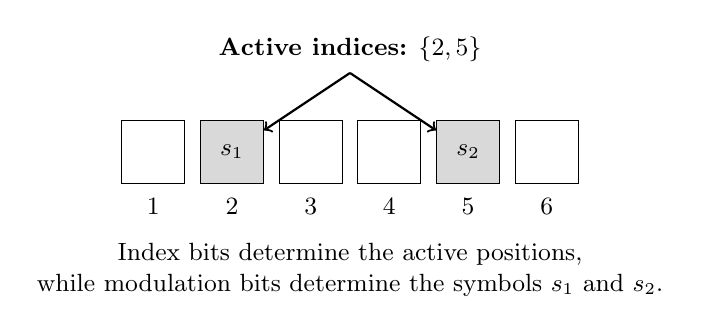
\begin{tikzpicture}[
    every node/.style={font=\small},
    active/.style={draw, fill=gray!30, minimum width=0.8cm, minimum height=0.8cm},
    inactive/.style={draw, minimum width=0.8cm, minimum height=0.8cm},
    arrow/.style={->, thick}
]

\node[align=center] at (2.5,1.3)
{\textbf{Active indices:} $\{2,5\}$};

\node[inactive] (r1) at (0,0) {};
\node[active]   (r2) at (1,0) {$s_1$};
\node[inactive] (r3) at (2,0) {};
\node[inactive] (r4) at (3,0) {};
\node[active]   (r5) at (4,0) {$s_2$};
\node[inactive] (r6) at (5,0) {};

\node at (0,-0.7) {\small 1};
\node at (1,-0.7) {\small 2};
\node at (2,-0.7) {\small 3};
\node at (3,-0.7) {\small 4};
\node at (4,-0.7) {\small 5};
\node at (5,-0.7) {\small 6};

\draw[arrow] (2.5,1.0) -- (r2);
\draw[arrow] (2.5,1.0) -- (r5);

\node[align=center] at (2.5,-1.5)
{Index bits determine the active positions,\\
while modulation bits determine the symbols $s_1$ and $s_2$.};

\end{tikzpicture}

\caption{Basic principle of index modulation using active resource elements.}
\label{fig:index_modulation_principle}
\end{figure}

As shown in Fig.~\ref{fig:index_modulation_principle}, only selected resource elements are activated in an IM-based transmission block. The receiver detects both the active indices and the transmitted constellation symbols in order to recover the original information bits.

\subsubsection{OFDM-IM Systems}

One of the most widely studied applications of Index Modulation is OFDM with Index Modulation (OFDM-IM). In conventional OFDM, all subcarriers are generally used to transmit constellation symbols. In OFDM-IM, however, only a subset of subcarriers within each subblock is activated, and the indices of these active subcarriers are used to convey additional information bits.

For an OFDM-IM subblock with \(n\) subcarriers, \(k\) active subcarriers, and \(M_{\mathrm{mod}}\)-ary modulation, the total number of transmitted bits per subblock is given by

\begin{equation}
p_{\mathrm{OFDM\text{-}IM}}
=
\left\lfloor \log_2 \binom{n}{k} \right\rfloor
+
k \log_2 M_{\mathrm{mod}}.
\end{equation}

The first term corresponds to the index bits, while the second term corresponds to the conventional modulation bits carried by the active subcarriers. Therefore, OFDM-IM can be viewed as an extension of OFDM in which subcarrier activation patterns introduce an additional information-carrying dimension.

\begin{figure}[H]
\centering

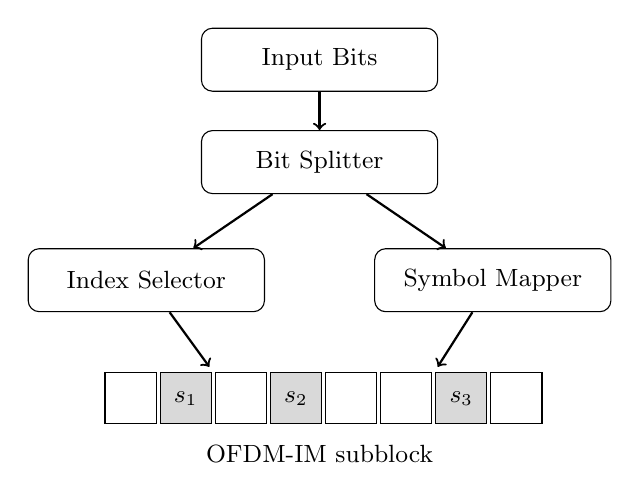
\begin{tikzpicture}[
    every node/.style={font=\small},
    block/.style={
        draw,
        rounded corners,
        minimum width=3.0cm,
        minimum height=0.8cm,
        align=center
    },
    arrow/.style={->, thick},
    active/.style={draw, fill=gray!30, minimum width=0.65cm, minimum height=0.65cm},
    inactive/.style={draw, minimum width=0.65cm, minimum height=0.65cm}
]

\node[block] (bits) at (0,0) {Input Bits};
\node[block] (split) at (0,-1.3) {Bit Splitter};
\node[block] (index) at (-2.2,-2.8) {Index Selector};
\node[block] (mapper) at (2.2,-2.8) {Symbol Mapper};

\draw[arrow] (bits) -- (split);
\draw[arrow] (split) -- (index);
\draw[arrow] (split) -- (mapper);

\node[inactive] (s1) at (-2.4,-4.3) {};
\node[active]   (s2) at (-1.7,-4.3) {$s_1$};
\node[inactive] (s3) at (-1.0,-4.3) {};
\node[active]   (s4) at (-0.3,-4.3) {$s_2$};
\node[inactive] (s5) at (0.4,-4.3) {};
\node[inactive] (s6) at (1.1,-4.3) {};
\node[active]   (s7) at (1.8,-4.3) {$s_3$};
\node[inactive] (s8) at (2.5,-4.3) {};

\node at (0,-5.0) {OFDM-IM subblock};

\draw[arrow] (index) -- (-1.4,-3.9);
\draw[arrow] (mapper) -- (1.5,-3.9);

\end{tikzpicture}

\caption{Conceptual structure of an OFDM-IM subblock.}
\label{fig:ofdm_im_subblock}
\end{figure}

The OFDM-IM concept provides a useful foundation for understanding more advanced IM-based systems. Since the present thesis focuses on OTFS-IM, the detailed mathematical design of OFDM-IM is not discussed extensively in this chapter. Instead, OFDM-IM is introduced as a representative example showing how index patterns can be exploited for information transmission.

\subsubsection{Advantages and Challenges of IM}

Index Modulation offers several attractive advantages for wireless communication systems. First, it provides an additional mechanism for conveying information without relying solely on constellation symbols. This can improve spectral efficiency or allow lower modulation orders to be used for a given transmission rate.

Second, IM offers flexibility in resource allocation. By changing the number of active resources, modulation order, and index mapping strategy, the system can be adapted to different performance requirements. For example, increasing the number of active resources may improve data rate, while reducing the number of active resources may reduce transmit energy and interference.

Third, IM can improve error performance in certain channel conditions because inactive resource elements provide additional structure that may assist detection at the receiver. The sparsity introduced by index activation can also be beneficial for receiver design, especially in systems where the channel itself has a sparse structure.

However, Index Modulation also introduces several challenges. The receiver must detect both the active indices and the transmitted symbols, which may increase detection complexity compared with conventional modulation. Furthermore, incorrect detection of active indices can lead to multiple bit errors because both index bits and symbol bits may be affected.

Another challenge is the design of efficient index mapping tables. Since the number of available activation patterns \(\binom{n}{k}\) is not always a power of two, only a subset of all possible patterns may be used in practical systems. This may lead to unused patterns and requires careful mapping design.

The main advantages and challenges of Index Modulation are summarized in Table~\ref{tab:im_advantages_challenges}.

\begin{table}[H]
\centering
\caption{Advantages and challenges of Index Modulation.}
\label{tab:im_advantages_challenges}

\small
\setlength{\tabcolsep}{6pt}
\begin{tabularx}{0.95\textwidth}{|>{\RaggedRight\arraybackslash}p{0.31\textwidth}|>{\RaggedRight\arraybackslash}X|}
\hline
\textbf{Aspect} &
\textbf{Description} \\
\hline

Additional information dimension &
Information is transmitted through both constellation symbols and active indices. \\
\hline

Flexible system design &
The number of active resources and modulation order can be adjusted according to system requirements. \\
\hline

Potential energy efficiency &
Only selected resources are active in each transmission block. \\
\hline

Detection complexity &
The receiver must jointly detect active indices and transmitted symbols. \\
\hline

Index detection errors &
Incorrect index detection may cause multiple bit errors. \\
\hline

Mapping design &
Efficient mapping is required when the number of activation patterns is not a power of two. \\
\hline

\end{tabularx}

\end{table}

In the context of this thesis, Index Modulation is considered as a promising technique to enhance OTFS transmission. The detailed OTFS-IM system model, including index mapping in the delay-Doppler domain, transmitter structure, receiver detection, and performance evaluation, will be presented in Chapter 4.
